\chapter{Red Black Tree}
A red-black tree is a special type of binary search tree with one extra bit of storage per node, its color which can be either red or black. Also, we keep the tree approximately balanced by enforcing some properties on the tree.
\begin{definition}{Perfect Binary Tree}{}
	It is a Binary Tree in which every internal node has exactly two children and all leaves are at the same level.
\end{definition}
\begin{Lemma}{}{}
	Every perfect binary tree with $k$ leaves has $2k-1$  nodes (i.e. $k-1$ internal nodes).
\end{Lemma}
\begin{definition}{Red Black Tree}{}
	\begin{minipage}{0.5\textwidth}
		A red-black tree is a binary tree with the following properties:
		\begin{itemize}
			\item Every internal node is key/NIL node. Every leaf is a ``NIL'' node.
			\item Each node (NIL and key) is colored either red or black.
			\item  Root and NIL nodes are always black.
			\item Any child of a red node is black.
			\item The path from root to any leaf has the same number of black nodes.
		\end{itemize}
	\end{minipage}\hfill
	\begin{minipage}{0.49\textwidth}
		\centering
		\usetikzlibrary{trees,arrows,positioning, calc}
		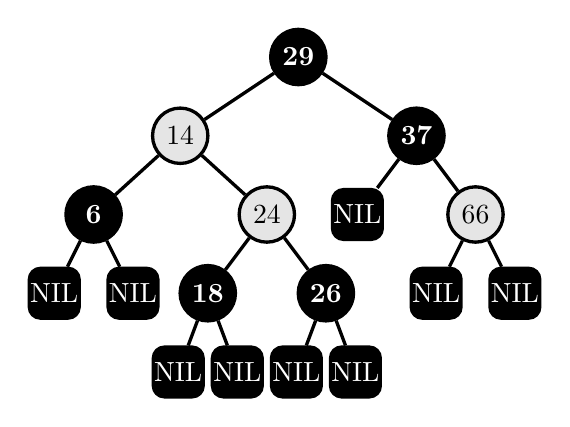
\begin{tikzpicture}[very thick,
				level/.style={sibling distance=30mm/#1},
				level distance=10mm,
				redVertex/.style={draw,fill=black!10!white,circle,minimum size=20pt,inner sep=0pt},
				blackVertex/.style={draw,fill=black,   circle,minimum size=20pt,inner sep=0pt, text=white, font=\bfseries},
				nil/.style={draw,fill=black,rectangle,rounded corners, minimum size=18pt,inner sep=0pt, text=white}]
			\node [blackVertex] (r){29}
			child {
					node[redVertex] {14}
					child [sibling distance=22mm] {
							node[blackVertex] {6}
							child {node [nil] {NIL}}
							child {node [nil] {NIL}}
						}
					child [sibling distance=22mm] {
							node [redVertex] {24}
							child [sibling distance=15mm] {
									node [blackVertex] {18}
									child {node [nil] {NIL}}
									child {node [nil] {NIL}}
								}
							child [sibling distance=15mm] {
									node [blackVertex] {26}
									child {node [nil] {NIL}}
									child {node [nil] {NIL}}
								}
						}
				}
			child {
					node[blackVertex] {37}
					child {node [nil] {NIL}}
					child {
							node [redVertex] {66}
							child {node [nil] {NIL}}
							child { node [nil] {NIL}}
						}
				};
		\end{tikzpicture}
		\captionof{figure}{A Red Black Tree}
		\label{fig:red-black-tree}
	\end{minipage}
\end{definition}

We call the number of black nodes on any simple path from  but not including a node $x$ down to a leaf the \emph{black-height} of the node, denoted by $bh(x)$. We generally confine our interest to the internal nodes of a red-black tree, since they hold the key values.
\begin{Lemma}{}{}
	A Red-Black Tree with $n$ internal nodes or key nodes has height at most $O(\log n)$.
\end{Lemma}
\begin{proof}
	We will first show that for any subtree rooted at node $x$ contains at least $2^{bh(x)}-1$ internal nodes. We will show this using induction on the height of the tree. For the base case let height of $x$ is $0$. Then $x$ must be a leaf. Therefore, the subtree rooted at $x$ has at least $bh(x)=0$. Hence, $2^{bh(x)}-1=2^0-1=0$  nodes which is true. For inductive step let $x$ has some positive height, and it is an internal node of the R-B Tree. Now $x$ has two children. Hence, each child has black-height either $bh(x)$ or $bh(x)-1$. By inductive hypothesis, the subtrees rooted at the children of $x$ have at least $2^{bh(x)-1}-1$ internal nodes. Thus, subtree rooted at $x$ has at least $2^{bh(x)-1}-1+2^{bh(x)-1}-1+1=2^{bh(x)}-1$ internal nodes.

	Now if the R-B tree has height $h$. Then any path from the root to a leaf at least half the nodes including the root must be black. So $bh(\emph{root})\geq \frac{h}2$. Thus, $n\geq 2^{\frac{h}2}-1\implies h\leq 2\log(n+1)$. Hence, we have the lemma.
\end{proof}
\nt{
	\begin{minipage}{0.3\textwidth}
		\centering
		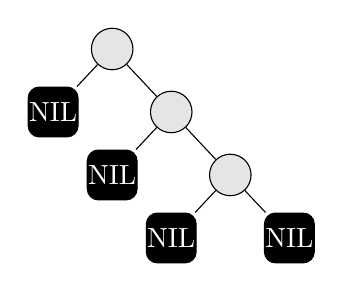
\begin{tikzpicture}[
				level distance=8mm,
				vertex/.style={draw,fill=black!10!white,circle,minimum size=15pt,inner sep=0pt},
				nil/.style={draw,fill=black,rectangle,rounded corners, minimum size=18pt,inner sep=0pt, text=white}
			]
			\node[vertex] (a) {}
			child { node [nil] {NIL} }
			child {
					node [vertex] (b) {}
					child { node [nil] {NIL} }
					child {
							node [vertex] (c) {}
							child { node [nil] {NIL} }
							child { node [nil] {NIL} }
						}
				};
		\end{tikzpicture}
	\end{minipage}\hfill
	\begin{minipage}{0.69\textwidth}
		Not all trees can be colored in a way that satisfies the properties of a red-black tree. Consider the following tree:\parinn

		In this example the root has to be black. The other two internal nodes can not be black since otherwise the path from the leaf of the root to root has only 2 black nodes but in the path from bottom most leaf to root will have 3. Then those two internal nodes has to be red. But that violates the property that a red node can not have a red child. Hence, this tree can not be colored in a way that satisfies the properties of a red-black tree.
	\end{minipage}
}

Since by the lemma the R-B tree has height at most $O(\log n)$ and it is a binary search tree we can perform search of a node using \textsc{Find} in $O(\log n)$ time. So now we will focus on the insertion and deletion operations in a red-black tree.  To insert or delete a node in a red-black tree we will  rotations to balance the tree again. So first we will visit rotations.
\section{Rotation}
A rotation is a local operation that changes the structure of a binary tree without violating the binary search tree property. There are two types of rotations: left rotation and right rotation.

When we do a left rotation on a node we assume that its right child is not NIL. The left rotation ``pivots'' around the link from the node to its right child and makes the right child the new root of the subtree with the ode as its left child.  Similarly, we can explain the right rotation. The rotations behave like the following:

\begin{figure}[!h]
	\centering
	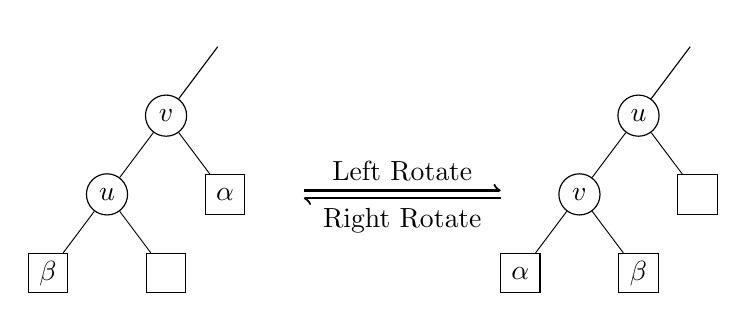
\begin{tikzpicture}[
			every node/.style={align=center, line width=0.15mm},
			level 1/.style={level distance=1cm, sibling distance=1.5cm},  % Adjusted distance for level 1
			level 2/.style={sibling distance=1.5cm},   % Adjusted distance for level 2
			square/.style={draw, shape=rectangle, minimum width=0.5cm, minimum height=0.5cm, inner sep=0pt, text width=0.5cm, text centered},
			circle/.style={draw, shape=circle, minimum width=0.5cm, minimum height=0.5cm, inner sep=0pt, text width=0.5cm, text centered},
			filled/.style={fill=white, , draw, line width=0.12mm},  % Style for filled nodes
			every edge/.style = {draw, latex'-latex' , line width=0.3mm, dotted,},
			parentarrow/.style={line width=0.12mm},  % Style for arrows from nodes to children
		]

		% Leftmost tree
		\node (AA0) {}
		child{
				node[circle] (A2) {$v$}
				child {node[circle] (B2) {$u$}
						child {node[square] (D2) {$\beta$} edge from parent[parentarrow]}
						child {node[square] (E2) {$\gm$} }
						edge from parent[parentarrow]
					}
				child {node[square,filled] (C2) {$\alpha$} edge from parent[parentarrow]}
			}
		child [missing] { node (AA5) {} };
		% Right tree
		\begin{scope}[shift={(6,0)}]
			\node (A0) {}
			child{
					node[circle] (A1) {$u$}
					child {node[circle] (B1) {$v$}
							child {node[square] (D1) {$\alpha$} edge from parent[parentarrow]}
							child {node[square] (E1) {$\beta$} }
							edge from parent[parentarrow]
						}
					child {node[square,filled] (C1) {$\gm$} edge from parent[parentarrow]}
				}
			child [missing] { node (A5) {} };

		\end{scope}

		\draw[thick, -left to] ($(C2)+(1,0.05)$) -- node[midway, above] {Left Rotate} ($(B1)+(-1,0.05)$);
		\draw[thick, -left to] ($(B1)+(-1,-0.05)$) -- node[midway, below] {Right Rotate}($(C2)+(1,-0.05)$)  ;
	\end{tikzpicture}
	\caption{Left and Right rotate about $u-v$}
\end{figure}\parinf

\begin{minipage}{0.46\textwidth}
	\begin{algorithm}[H]
	\caption{\textsc{Left-Rotate}$({T,x})$}
	\DontPrintSemicolon
	$y\longleftarrow x.\emph{right}$\;
	$x.\emph{right}\longleftarrow y.\emph{left}$\;
	\If{$y.\emph{left}\neq \emph{NIL}$}{
		$y.\emph{left}.\emph{parent}\longleftarrow x$\;
	}
	$y.\emph{parent}\longleftarrow x.\emph{parent}$\;
	\If{$x.\emph{parent}==\emph{NIL}$}{
		$T.\emph{root}\longleftarrow y$\;
	}
	\ElseIf{$x== x.\emph{parent}.\emph{left}$}{
		$x.\emph{parent}.\emph{left}\longleftarrow y$\;
	}
	\Else{
		$x.\emph{parent}.\emph{right}\longleftarrow y$\;
	}
	$y.\emph{left}\longleftarrow x$\;
	$x.\emph{parent}\longleftarrow y$
\end{algorithm}
\end{minipage}\hfill
\begin{minipage}{0.46\textwidth}
	\begin{algorithm}[H]
		\caption{\textsc{Right-Rotate}$({T,x})$}
		\DontPrintSemicolon
		$y\longleftarrow x.\emph{left}$\;
		$x.\emph{left}\longleftarrow y.\emph{right}$\;
		\If{$y.\emph{right}\neq \emph{NIL}$}{
			$y.\emph{right}.\emph{parent}\longleftarrow x$\;
		}
		$y.\emph{parent}\longleftarrow x.\emph{parent}$\;
		\If{$x.\emph{parent}==\emph{NIL}$}{
			$T.\emph{root}\longleftarrow y$\;
		}
		\ElseIf{$x== x.\emph{parent}.\emph{left}$}{
			$x.\emph{parent}.\emph{left}\longleftarrow y$\;
		}
		\Else{
			$x.\emph{parent}.\emph{right}\longleftarrow y$\;
		}
		$y.\emph{right}\longleftarrow x$\;
		$x.\emph{parent}\longleftarrow y$
	\end{algorithm}
\end{minipage}\parinn

Both \textsc{Left-Rotate} and \textsc{Right-Rotate} take $O(1)$ time. Only some constantly many pointers are changed by rotation all other attributes in a node remain the same. 
\section{Insertion}
We will now describe how to insert a node in a red-black tree in $O(\log n)$ time. We will insert the node in the tree in place of a leaf replacing a NIL node. After that we will color the node red and then use rotations to increase the height of the node at each iteration until the properties of a red-black tree are satisfied. 

Let the node added is $v$. We define the attribute \emph{uncle} which is basically sibling of the parent. Since at the time of addition we coloring the node red it is not hampering the number of black nodes in the path from root to any leaf. So only time it violates the properties of a red-black tree is when the parent of the node is red. Now two cases can happen:
\begin{enumerate}[label=Case \Roman*:, leftmargin=*]
	\item $v.\emph{uncle}.color$=Red: Then $v.\emph{parent}.\emph{parent}$  is black. 
	\begin{figure}[!h]
	\centering
	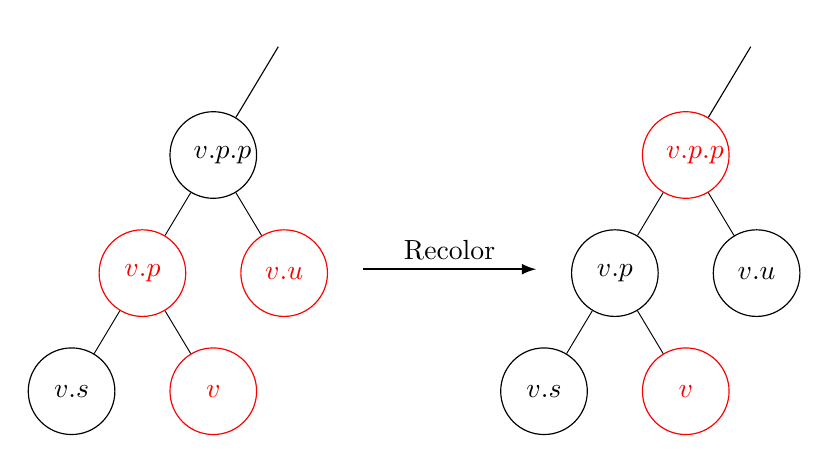
\begin{tikzpicture}[
			every node/.style={align=center, line width=0.15mm},
			level 1/.style={level distance=1.5cm, sibling distance=1.8cm},  % Adjusted distance for level 1
			level 2/.style={sibling distance=1.8cm},   % Adjusted distance for level 2
			redVertex/.style={draw, shape=circle, minimum width=1.1cm, minimum height=0.5cm, inner sep=0pt, text width=0.5cm, text centered, text=red!75!black, color=red},
			blackVertex/.style={draw, shape=circle, minimum width=1.1cm, minimum height=0.5cm, inner sep=0pt, text width=0.5cm, text centered},
			every edge/.style = {draw, latex'-latex' , line width=0.3mm, dotted,},
			Rparentarrow/.style={line width=0.12mm, color=red},  % Style for arrows from nodes to children
			parentarrow/.style={line width=0.12mm}
		]

		% Leftmost tree
		\node (AA0) {}
		child{
				node[blackVertex] (A2) {$v.p.p$}
				child {node[redVertex] (B2) {$v.p$}
						child {node[blackVertex] (D2) {$v.s$} edge from parent[parentarrow]}
						child {node[redVertex] (E2) {$v$} }
						edge from parent[parentarrow]
					}
				child {node[redVertex] (C2) {$v.u$} edge from parent[parentarrow]}
			}
		child [missing] { node (AA5) {} };
		% Right tree
		\begin{scope}[shift={(6,0)}]
			\node (A0) {}
			child{
					node[redVertex] (A1) {$v.p.p$}
					child {node[blackVertex] (B1) {$v.p$}
							child {node[blackVertex] (D1) {$v.s$} edge from parent[parentarrow]}
							child {node[redVertex] (E1) {$v$} }
							edge from parent[parentarrow]
						}
					child {node[blackVertex] (C1) {$v.u$} edge from parent[parentarrow]}
				}
			child [missing] { node (A5) {} };

		\end{scope}

		\draw[thick, -latex] ($(C2)+(1,0.05)$) -- node[midway, above] {Recolor} ($(B1)+(-1,0.05)$);
	\end{tikzpicture}
\end{figure}
In this case we can recolor $v.\emph{parent}.\emph{parent}$ to red and both $v.\emph{parent}$ and $v.\emph{uncle}$ to be black. This will preserve the number of black nodes in any simple path from root to any leaf. 
\end{enumerate}